\documentclass{beamer}

\usepackage{beamerthemesplit}
\usepackage{amsmath}
\usepackage{amsfonts}
\usepackage{amssymb}
\usepackage{qtree}
\usepackage{cancel}
\usepackage{tkz-graph}
%\usepackage[pdftex]{graphicx}

\mode<presentation>
{
  \usetheme{Warsaw}
  % or ...

  %\setbeamercovered{transparent}
  % or whatever (possibly just delete it)
}


\usepackage[english]{babel}
% or whatever

\usepackage[latin1]{inputenc}
% or whatever

\usepackage{times}
\usepackage[T1]{fontenc}

\title{Controlling Intelligent Agents in Virtual World}

\subtitle{The OpenCog Embodiment Component}

\author{Nil Geisweiller}

\institute[Xiamen University] % (optional, but mostly needed)
{
  Novamente LLC
}

\date[Xiamen University AGI Summer School 2009] % (optional, should be abbreviation of conference name)
{Xiamen University\\ AGI Summer School 2009}


\AtBeginSection[]
{
  \begin{frame}<beamer>{Outline}
    \tableofcontents[currentsection,currentsection]
  \end{frame}
}

\AtBeginSubsection[]
{
  \begin{frame}<beamer>{Outline}
    \tableofcontents[currentsection,currentsubsection]
  \end{frame}
}

%\newcommand{\AND}{\textit{AND}}
%\newcommand{\OR}{\textit{OR}}
%\newcommand{\NOT}{\textit{NOT}}
\newcommand{\AND}{\land}
\newcommand{\OR}{\lor}
\newcommand{\NOT}{\lnot}


\begin{document}

\frame
{
  \maketitle
}
\section[Outline]{}
\frame{\tableofcontents}

\section{Introduction}

\frame
{

  \frametitle{What is Opencog Embodiment Component?}
  
  \begin{beamerboxesrounded}{Embodiment component (formerly called PetBrain)}
    Interface OpenCog for virtual world agents or robots
  \end{beamerboxesrounded}
  
 \begin{columns}
    \column{0.5in}
    
\includegraphics[scale=0.6]{cog-big.png}
    \column{2in}
    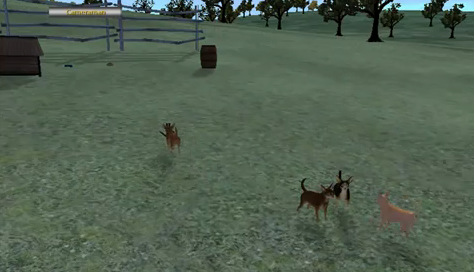
\includegraphics[scale=0.5]{petBrain_multiverse.png}
    \column{0.5in}
    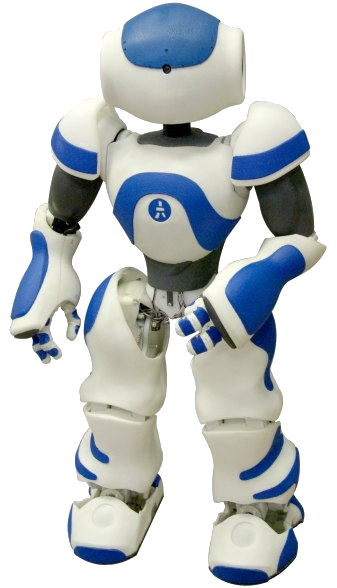
\includegraphics[scale=0.2]{nao-robot-791451.png}
 \end{columns}

%  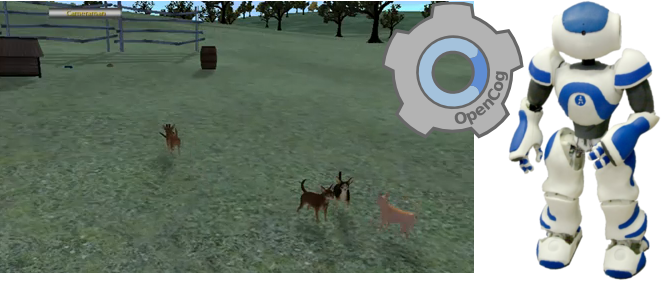
\includegraphics[scale=0.5]{EmbodimentSym.png}

}

\frame
{

  \frametitle{Embodiment Component Function}

  Goals:
  \begin{itemize}
  \item<+-> Environment where to teach and test OpenCog
  \item<+-> Virtual World $\Rightarrow$ Easier than real world
  \item<+-> But robot interface as well (in development)
  \end{itemize}

}


\frame
{
  \frametitle{Embodiment Component Overview}
  \begin{center}
    \includegraphics[scale=0.3]<1>{EmbodimentSystemArchitecture_0.png}
    \includegraphics[scale=0.3]<2>{EmbodimentSystemArchitecture_1.png}
    \includegraphics[scale=0.3]<3>{EmbodimentSystemArchitecture_2.png}
    \includegraphics[scale=0.3]<4>{EmbodimentSystemArchitecture_3.png}
    \includegraphics[scale=0.3]<5>{EmbodimentSystemArchitecture_4.png}
    \includegraphics[scale=0.3]<6>{EmbodimentSystemArchitecture_Com.png}
  \end{center}

  \pause

  \begin{enumerate}
  \item<+-> Proxy, \alert{interface between the virtual world and Embodiment}
  \item<+-> Operational Agent (Pet) Controller (OPC), \alert{reactive brain}
  \item<+-> Learning Server (LS), \alert{imitation learning for now}
  \item<+-> Collective Experience Store (CES) (not implemented yet)
  \item<+-> Router: communication with Sockets (distributed or not)
  \end{enumerate}
}

\section{Embodiment Sub-components}

\subsection{Proxy}

\frame{
  \frametitle{Embodiment Proxy}
  \begin{center}
  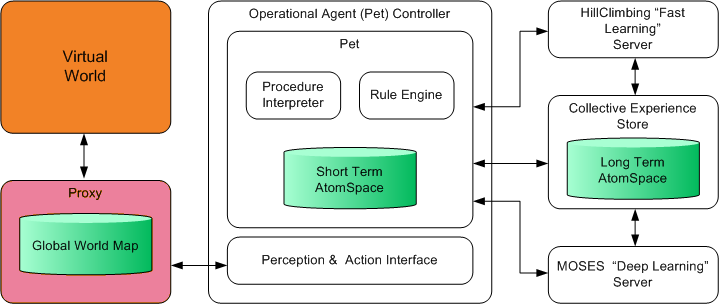
\includegraphics[scale=0.3]{EmbodimentSystemArchitecture_1.png}
  \end{center}

  \begin{beamerboxesrounded}{Proxy main function}
    Abstract away all details of interacting with a Virtual World
  \end{beamerboxesrounded}

}

\frame
{
  \frametitle{For the moment Embodiment Proxy for}

  \begin{itemize}
  \item<+-> Multiverse (implemented)
    
\includegraphics[scale=0.2]{multiverse_logo_large.jpg}
  \item<+-> realXtend (almost complete)
    
\includegraphics[scale=0.5]{realXtend_logo.jpg}
  \item<+-> Nao Robot (in development)
    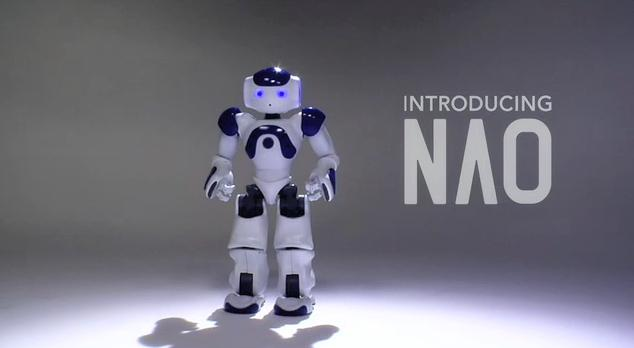
\includegraphics[scale=0.2]{nao_logo.jpg}
  \end{itemize}
}

\frame
{
  \frametitle{Embodiment Proxy sub-functions}

  Proxy handles:
  \begin{itemize}
  \item<+-> Input stream of \alert{perceptual data}
  \item<+-> Output stream of \alert{actions and action feedback}
    ({\tt failure} or {\tt success})
 \item<+-> Maintaining a Global World Map (GWM)
   \begin{itemize}
   \item Shared GWM for all agents\\ $\Rightarrow$ reduce message traffic
     agents $\leftrightarrow$ virtual world
   \end{itemize}
  \item<+-> Commands from a human avatar
    \begin{itemize}
    \item messages to the agents, order, queries
    \item meta-commands (load agent, etc)
    \end{itemize}
  \end{itemize}
}

\frame
{
  \frametitle{Embodiment Proxy $\leftrightarrow$ PAI}
  \begin{center}
  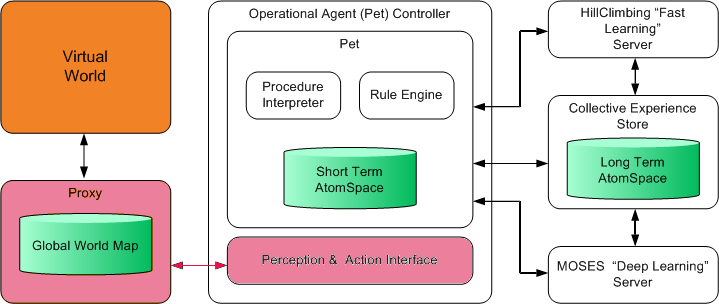
\includegraphics[scale=0.3]{EmbodimentSystemArchitecture_Proxy_PAI.png}
  \end{center}
  
  Proxy communicates with the OPC by the intermediate of the
  \alert{Perception Action Interface}.

}

\subsection{Operational Agent (Pet) Controller}

\frame
{
  \frametitle{Perception Action Interface Function}

  \begin{center}
    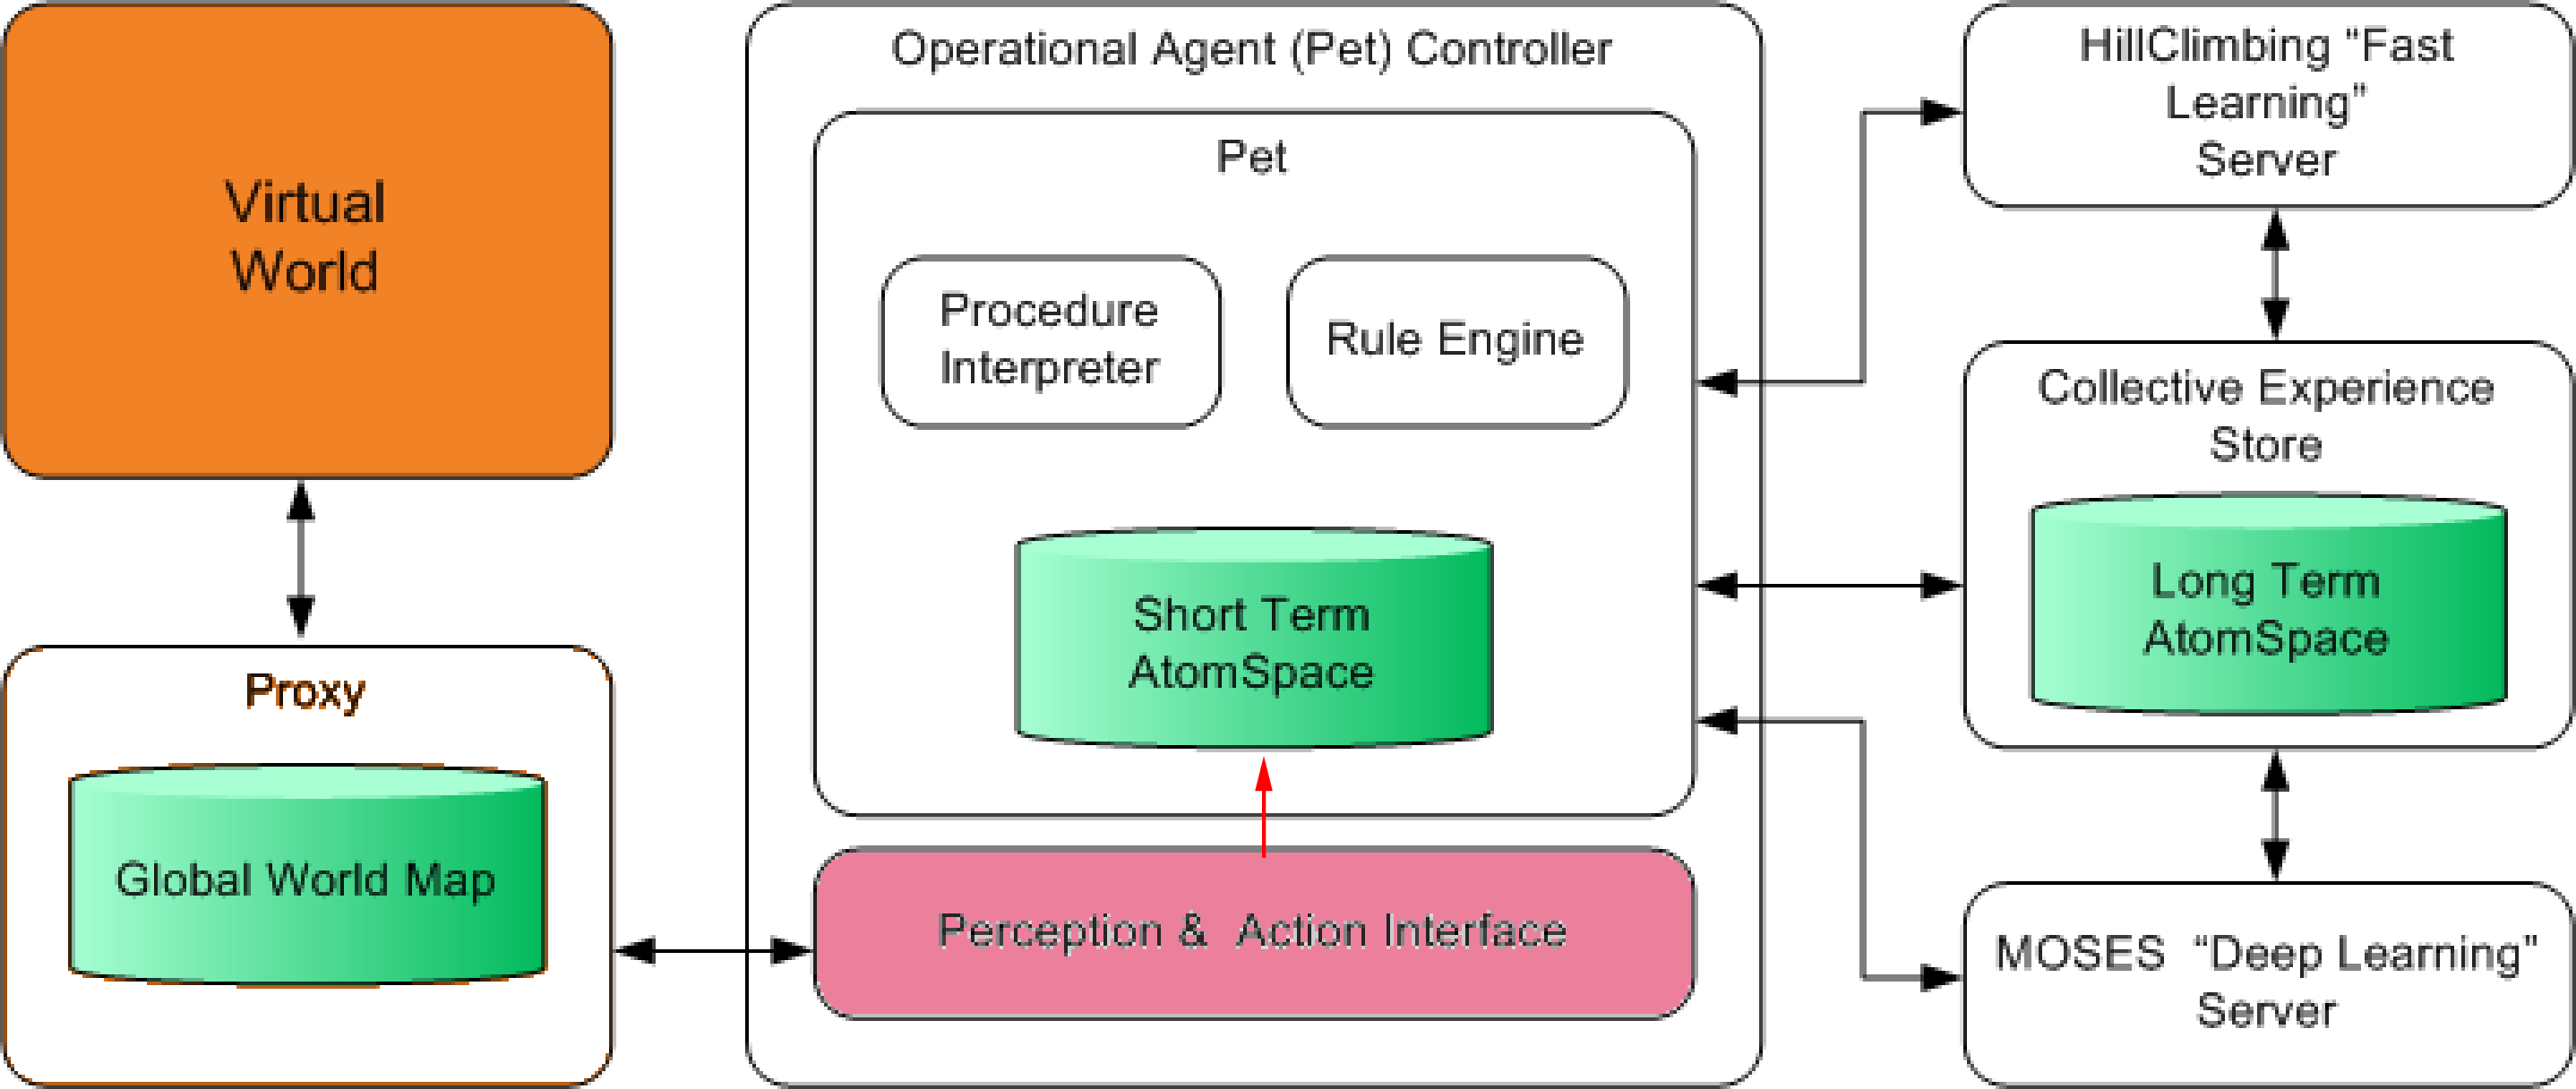
\includegraphics[scale=0.1]{Embodiement_PAI_OPC.png}
  \end{center}
  
  \begin{itemize}
  \item<+-> Convert Perceptions coming from the Proxy into \alert{atoms
    in the agent's atomSpace}
  \end{itemize}

}

\frame[containsverbatim]
{
  \frametitle{Perception Action Interface, perception $\rightarrow$ atoms}

  \begin{columns}

    \column{1in}
    
    % \begin{figure}
    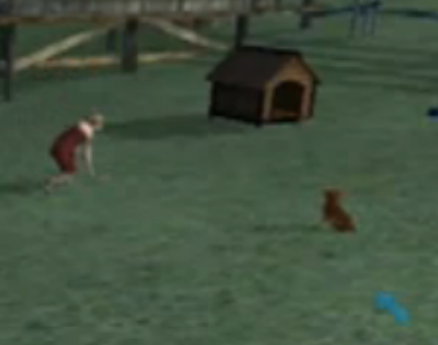
\includegraphics[scale=0.23]{grab_ball.png}
    % \caption{Pet watching avatar grabbing ball}
    % \end{figure}
    
    
    \column{1.5in}

    $\Rightarrow$ Proxy $\Rightarrow$ PAI $\Rightarrow$
    \column{2in}
    
{\tiny
\begin{verbatim}
AtTimeLink
    TimeNode: "15:32:24.182"
    EvaluationLink
        PredicateNode: "actionDone"
        ListLink
            AvatarNode: "owner"
            Node: "grab"
            ListLink
                ObjectNode: "ball_id"
\end{verbatim}
}

  \end{columns}

  \begin{enumerate}
  \item Pet watches the avatar grabbing a ball
  \item Proxy sends perception to PAI
  \item PAI writes the perception into the Pet's atomSpace
  \end{enumerate}
}

\frame
{
  \frametitle{Embodiment AtomSpace Extensions, \alert{Space and Time servers}}

  \only<1>{\includegraphics[scale=0.025]{bmp_grid.pdf}}
  \only<2->{\includegraphics[scale=0.025]{episodic_grid.pdf}}

  \begin{itemize}
  \item<+-> Space Server: SpaceMap wrapped in atom,
    associative container for fast retreival.
    \begin{itemize}
    \item SpaceMap:
      \begin{itemize}
      \item 2D Grid
      \item Objects inside
      \item Spacial functions and predicates, {\tt distance}, {\tt near}, 
        $\ldots$
      \end{itemize}
    \end{itemize}
  \item<+-> Time Server: indexing timestamped atoms for fast retrieval
  \end{itemize}

  \begin{center}
    \visible<2->{\alert{Episodic memory}}
  \end{center}
}

\frame
{
  \frametitle{Combo interpreter actions to action plan}

  \begin{center}
    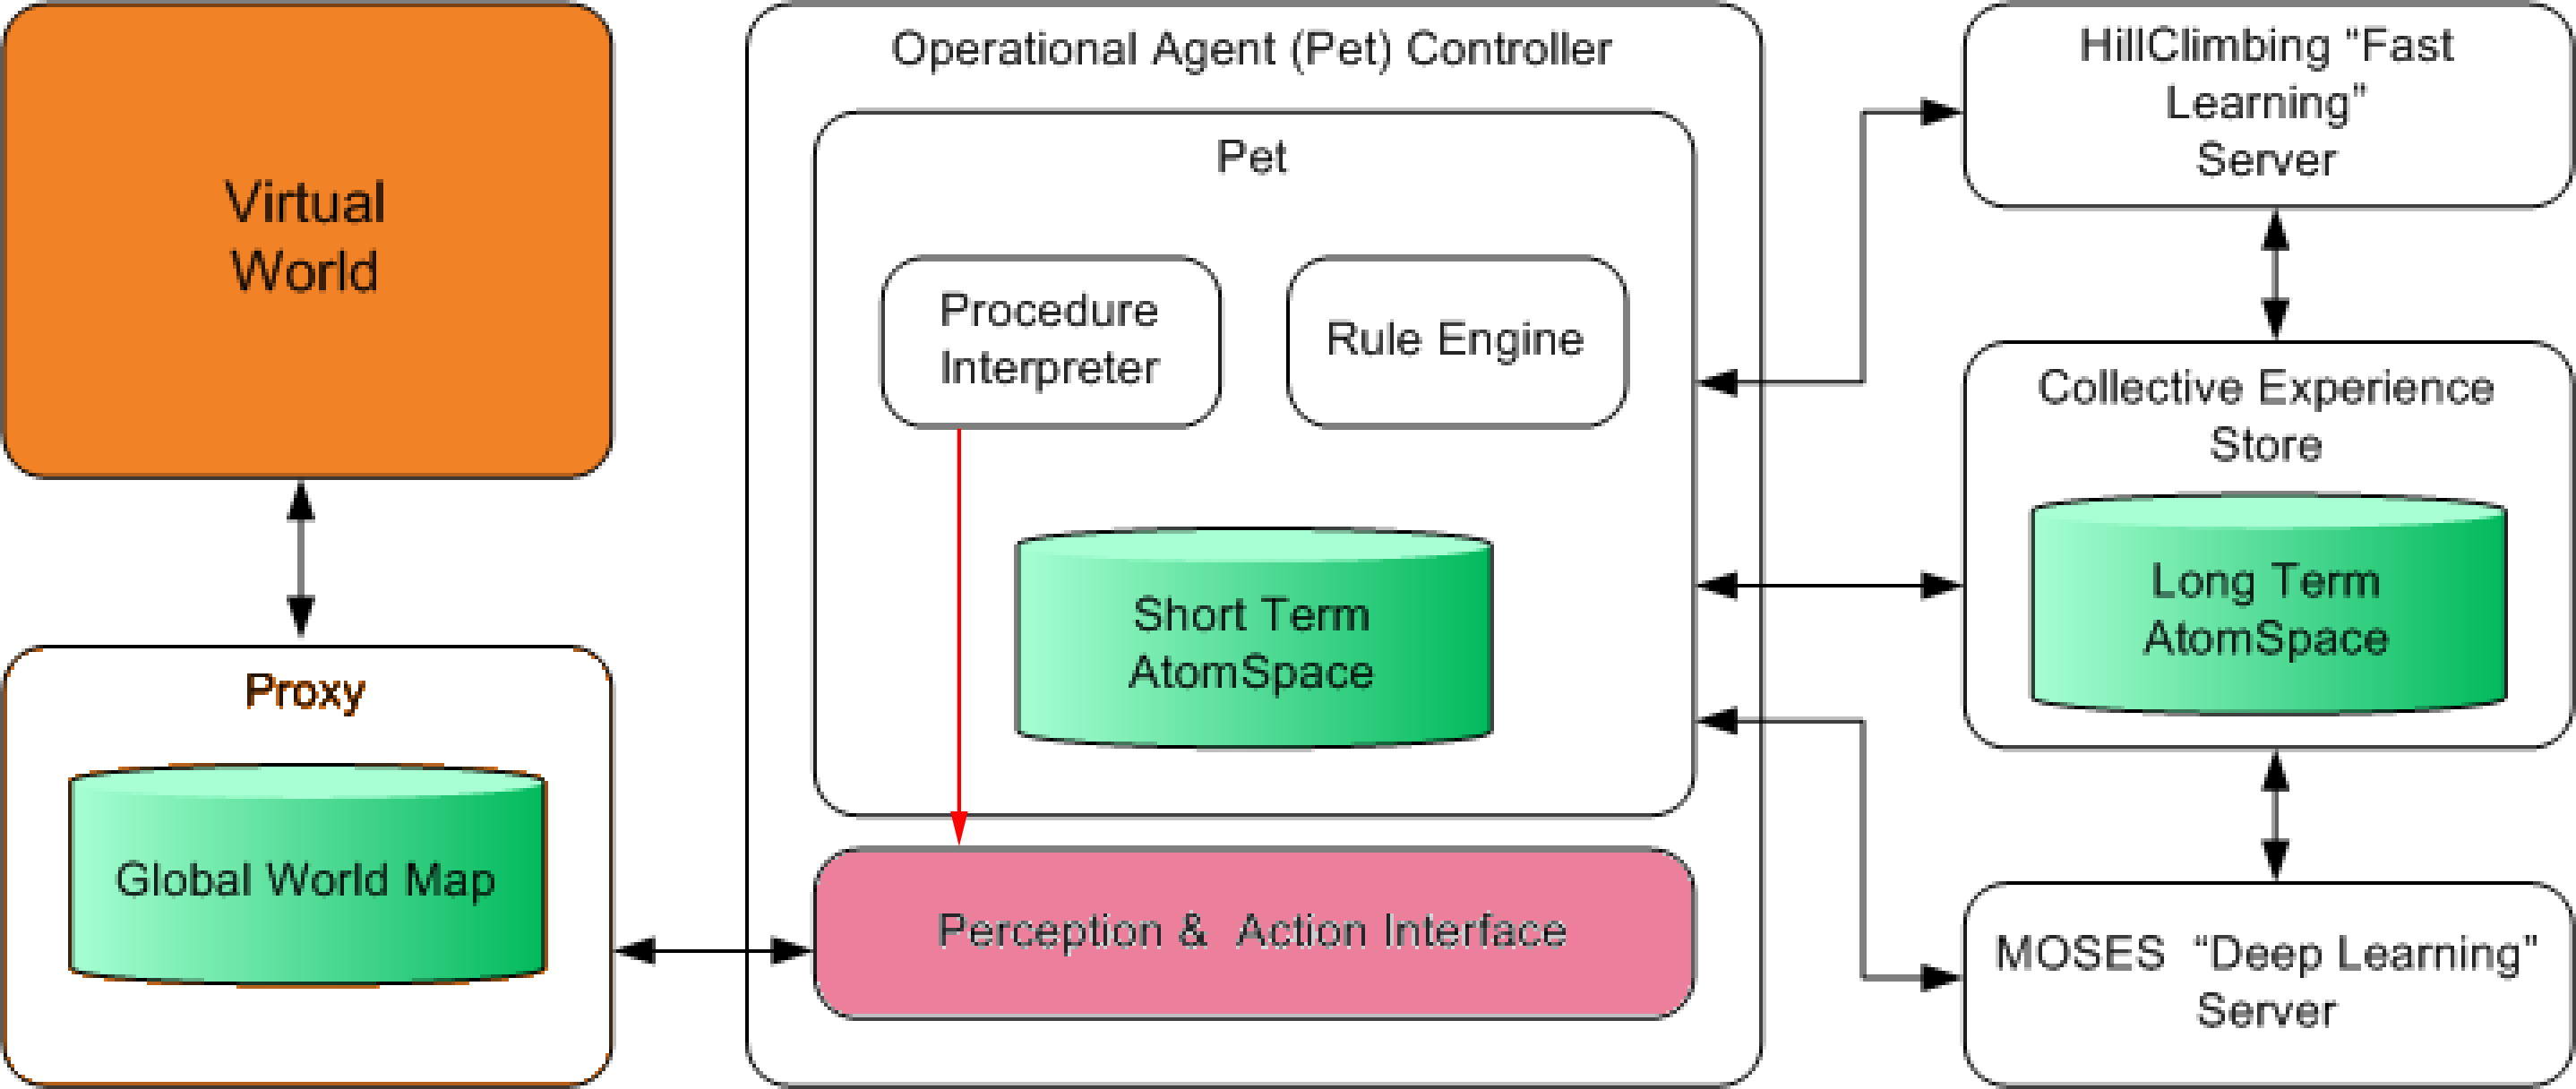
\includegraphics[scale=0.1]{Embodiment_Interpreter_PAI.png}
  \end{center}

  \begin{itemize}
  \item<+-> Convert actions coming from the \alert{Combo interpreter into action
    plans} (sequence of actions) to the Proxy
  \end{itemize}
}

\frame
{
  
  \frametitle{Combo interpreter actions to action plan}
  \begin{center}
    {\tt goto\_obj(barrel2)}\\
    PAI$\Downarrow$\\
%    Combo interpreter+PAI\\
%    $\Downarrow$\\
    {\tt \{walk(546, 453), walk(547, 451), ...\}}\\
    Proxy$\Downarrow$\\
    
    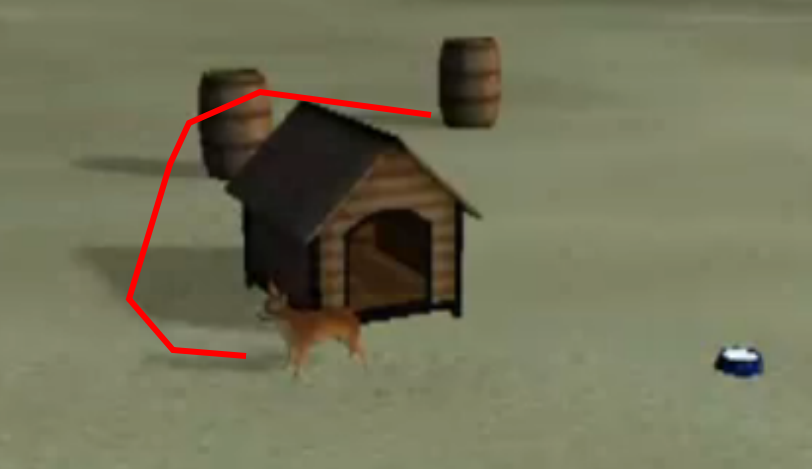
\includegraphics[scale=0.23]{goto_barrel.png}
  \end{center}

  \begin{enumerate}
    \item Combo interpreter + PAI create action plan
    \item PAI sends it to Proxy, which sends it to virtual world
    \end{enumerate}

}

\frame
{
  \frametitle{Rule Engine}

  \begin{center}
    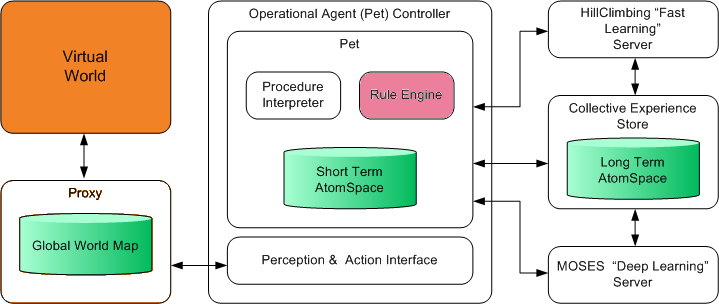
\includegraphics[scale=0.3]{Embodiment_RuleEngine.png}
  \end{center}

  \begin{beamerboxesrounded}{Rule Engine Function}
    \begin{itemize}
    \item<+-> Update agent's internal state. Example pet:
      \begin{itemize}
      \item agent's feeling (hunger, happiness, $\ldots$)
      \item agent's relation (familiar\_with, friend\_of, $\ldots$)
      \end{itemize}
    \item<+-> Select next action to \alert{satisfy its goals}. Example pet:
      \begin{itemize}
      \item Fulfill needs (hunger, thirst, curiosity, etc)
      \end{itemize}
    \end{itemize}
  \end{beamerboxesrounded}
    
}
  
\frame
{
  \frametitle{Rule Engine, how it works?}

  For the moment it is really crude!

  \begin{beamerboxesrounded}{Rule Engine: Main loop}
    Evaluates a set of hard-coded rules to update state and
    choose next actions.\\
    
    \pause
    
    3 types of rules:
    \begin{enumerate}
    \item<+-> Feeling rule\\
      {\footnotesize
      {\tt has\_eaten(self) $\Rightarrow$ happiness<0.8>}\\
      }
    \item<+-> Relation rule\\
      {\footnotesize
      {\tt has\_licked(self X) $\Rightarrow$ familiar\_with(self X)<0.9>}\\
      }
    \item<+-> Schema rule\\
      {\footnotesize
      {\tt is\_hungry(self) $\overset{0.6}{\Rightarrow}$ goto\_find\_food()}\\
      }
    \end{enumerate}
  \end{beamerboxesrounded}
}

\frame
{
  \frametitle{Rule Engine, how it works?}
  
  For the petBrain we have \alert{over 100 hard-coded rules!}
  \begin{itemize}
  \item 21 feeling rules
  \item 10 relation rules
  \item 76 schema rules
  \end{itemize}

  \alert{+ rule to use tricks learned by imitation}
}

\subsection{Learning Server}

\frame
{
  \frametitle{Learning Server}

  \begin{center}
    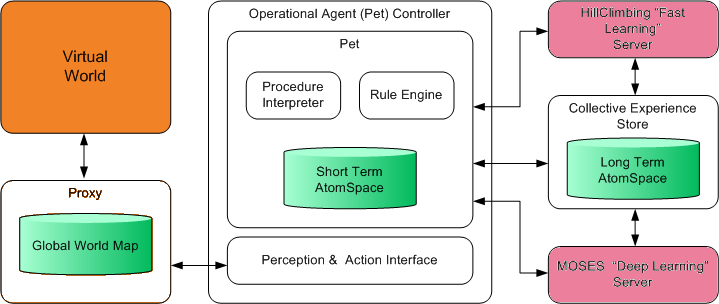
\includegraphics[scale=0.3]{EmbodimentSystemArchitecture_3.png}
  \end{center}

  \begin{beamerboxesrounded}{Lerning Server (LS) Function}
    Complex learning tasks (like imitation learning) run seperatly
    to not pertubate the agent's reactivity.
  \end{beamerboxesrounded}

  \begin{itemize}
  \item<+-> Imitation Learning (Implemented)
  \item<+-> Spontaneous Learning (not Implemented)
  \end{itemize}
}

\frame
{
  \frametitle{Imitation Learning}

  \begin{columns}

    \column{1.2in}
    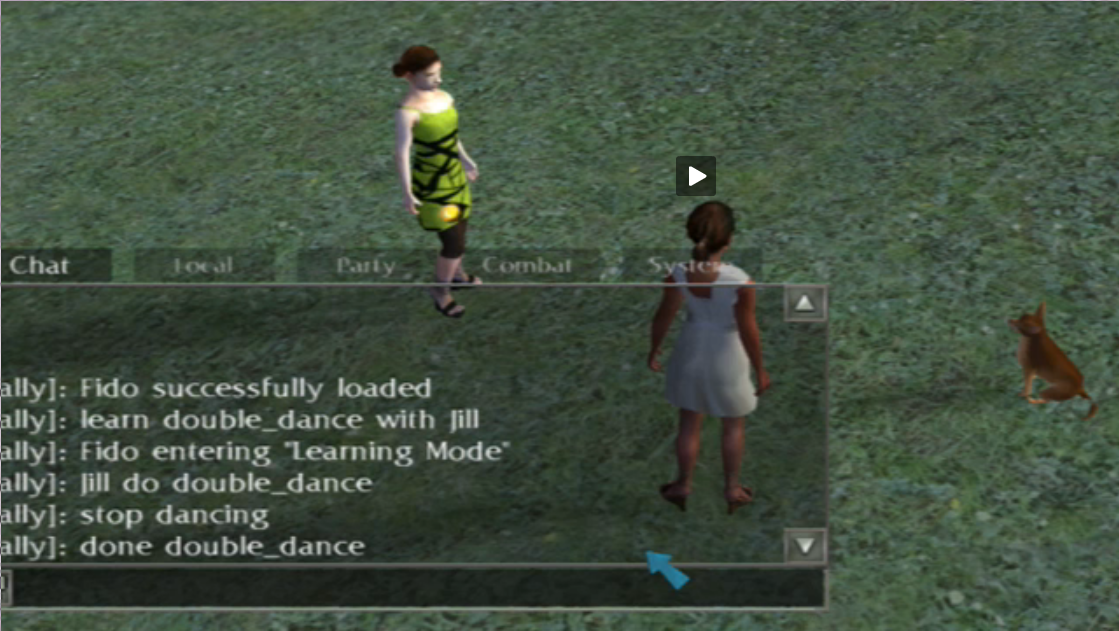
\includegraphics[scale=0.15]{double_dance.png}
    
    \column{2in}
    \visible<2->{
      \includegraphics[scale=0.15]<2>{episodic_memory_LS.png}
      \includegraphics[scale=0.15]<3->{search_combo_LS.png}
    }
  \end{columns}

  \begin{enumerate}
  \item<+-> Pet's owner requests \alert{learning session and shows the trick}
  \item<+-> OPC sends portion of atomSpace, \alert{episodic memory of the
    learning session to LS}
  \item<+-> LS searches a \alert{Combo program that mimics that trick}
    (using Hillclimbing or MOSES)
  \item<+-> Each Combo candidate is \alert{run inside the imaginary world}
    of that episodic memory, the result is
    \alert{compared with the avatar's behavior}
  \end{enumerate}
  
}

\frame
{
  \frametitle{Imitation Learning}

  \begin{columns}

    \column{1.2in}
    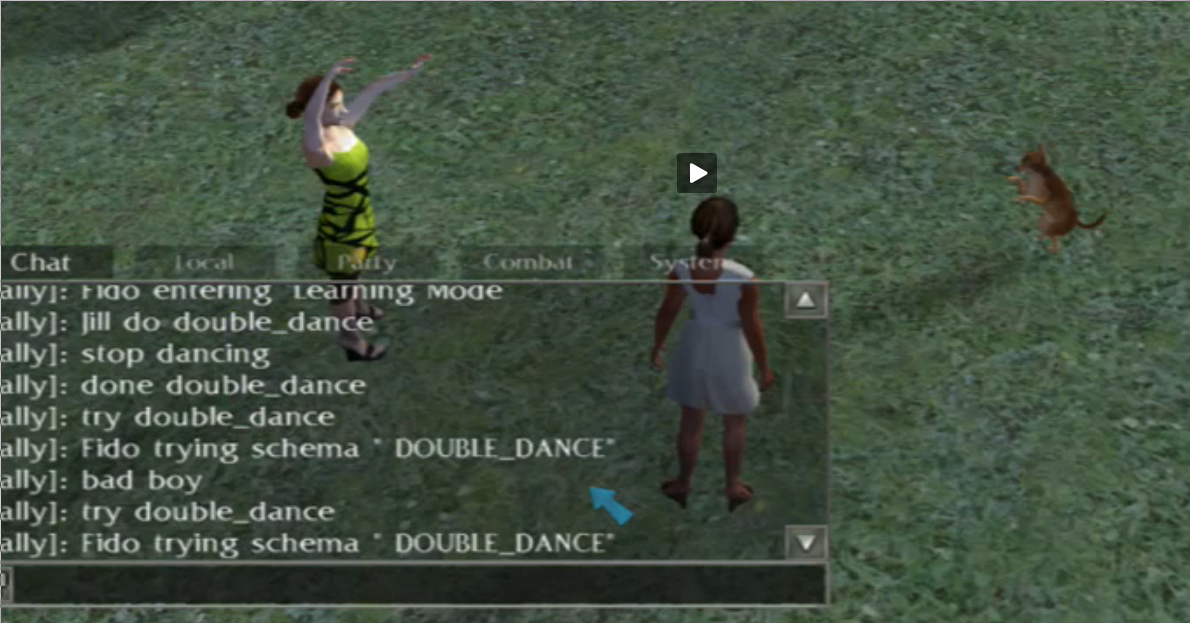
\includegraphics[scale=0.15]{try_trick.png}
    
    \column{1.7in}
    \visible<2>{
      \includegraphics[scale=0.15]<1,2>{return_combo.png}
    }
    \includegraphics[scale=0.15]<3->{return_combo_reward.png}
  \end{columns}

  \begin{enumerate}
  \item<+-> Owner asks the pet to \alert{try the trick}
  \item<+-> LS sends its \alert{best candidate so far},
    and pet execute the trick
  \item<+-> Owner sends \alert{positive or negative reward to guide} the
    search
  \end{enumerate}

}

\frame[containsverbatim]
{
  \frametitle{Example of trick learning: Double dance}

  Dance in loop on cue
  \begin{itemize}
  \item Owner kicks left leg $\Rightarrow$ tap dance
  \item Owner kicks right leg $\Rightarrow$ lean rock dance
  \end{itemize}

  \begin{beamerboxesrounded}{Combo to learn}
    {\small
\begin{verbatim}
boolean_while(not(says(owner "stop dancing"))
              action_if(last_action(owner "kickL")
                        tap_dance
                        lean_rock_dance))
\end{verbatim}
    }
  \end{beamerboxesrounded}
}

\subsection{Collective Experience Store}

\frame
{
  \frametitle{Collective Experience Store (not implemented yet)}

  \begin{center}
    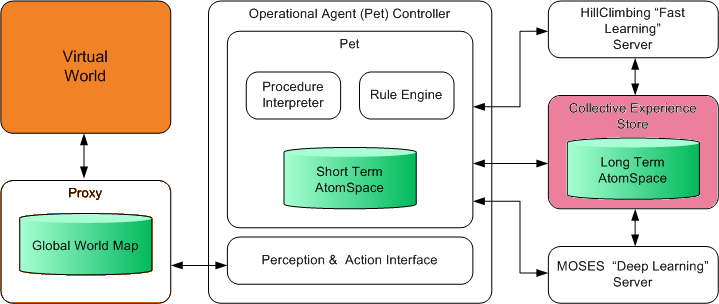
\includegraphics[scale=0.3]{EmbodimentSystemArchitecture_4.png}
  \end{center}

  \begin{beamerboxesrounded}{Collective Consciousness}
    All agents can put in common their knowledge. When one gets smarter
    everybody takes advantage of it.
  \end{beamerboxesrounded}

}

\section{Demo...}

\section{Conclusion}

\frame
{
  \frametitle{Conclusion}

   \begin{beamerboxesrounded}{What \alert{has been done}:}
     \begin{itemize}
     \item \alert{Hard-coded} behaviors
     \item Imitation learning
     \item but \alert{no spontaneous learning}
     \item No language understanding yet (only commands)
     \end{itemize}
   \end{beamerboxesrounded}
 }

 \frame
 {
   \frametitle{Conclusion}

  \begin{beamerboxesrounded}{What \alert{remains to be done}:}
    \begin{itemize}
    \item Spontaneous learning, concept creation, integrate Attention Allocation
    \item Transfer learning, Collective Experience Store
    \item Natural language processing and generation (in development)
    \end{itemize}
  \end{beamerboxesrounded}
 }

\end{document}
